\documentclass[a4paper]{article}
\usepackage{amssymb}
\usepackage{bbm}
\usepackage[normalem]{ulem}
\usepackage{graphicx}
\usepackage[colorlinks,linkcolor=blue,anchorcolor=blue,citecolor=blue,urlcolor=blue]{hyperref}
\usepackage{mciteplus}
\usepackage{etoolbox}
\usepackage{subcaption}
\usepackage{tikz}
\usetikzlibrary{shapes}
\usepackage{fontspec}

\title{Statement of Research}
\author{JinGuo Liu\\ Department of Physics, Harvard University}
\date{\today}

\newcommand{\<}{\langle}
\renewcommand{\>}{\rangle}
\newcommand{\vsigma}{\vec{\sigma}}
\setlength{\topmargin}{-10mm}
\setlength{\textwidth}{7in}
\setlength{\oddsidemargin}{-8mm}
\setlength{\textheight}{9in}
\setlength{\footskip}{1in}

\newfontfamily\DejaSans{DejaVu Sans}

\begin{document}
\fontsize{10}{13}
\selectfont
\maketitle

I am a Post-Doctoral Fellow in Mikhail Lukin's group at the department of physics at Harvard University with an interest in understanding the connection between computing and physics.
In the past decades, these two seemingly unrelated fields are more and more inter-weaved.
It brings many beautiful theories that deepened our understanding about the nature of computing and the nature of our physical world.
For example, 
%Another example is recent advances in understanding the hardness of problems from the overlap gap properties that highly inspired from the phase transition in spin glasses.
by relating the energy consumption in computation and a quantum system with environment, researchers showed why the Landauer's principle (every irreversible operation to a bit requires dissipating an energy lower bounded by $k_bT\ln 2$ to the environment) is true with a simple open quantum model~\cite{Reeb2014};
by relating the dynamics of a local Hamiltonian with a universal quantum Turing machine, researchers show the problem of telling whether a local Hamiltonian or an initial state thermalize or not is uncomputable~\cite{Shiraishi2021}, i.e. as hard as the famous halting problem in computer science.

The majority of my current research is also about relating computing and physics.
In the following, I will explain my past works mainly from two aspects, one is understanding the computational hardness from the solution space properties, another is embedding computational hard problems to a physical system.

\section{Solution space properties of hard combinatorial optimization problems}
\subsection{Current Work}
My first project in Harvard is to understand an experiment that uses variational quantum algorithms to solve the maximum independent set problem by embedding a problem instance into a Rydberg atom array Hamiltonian.
To explain why our quantum algorithm works better than classical simulated annealing in some graph instances but not in others,
I and my collaborators created a unified framework to solve the \textit{solution space properties} of a class of hard combinatorial optimization problems. Here, the solution space property refers to a class of quantities that not only include the maximum or minimum set size, but also include the number of sets at a give size, enumeration of all sets at a give size and direct sampling of such sets when they are too large to be fit into a memory; the class of problem includes but is not limited to the independent set problem, the maximum cut problem, the vertex coloring problem, the maximal clique problem, the dominating set problem, and the satisfiability problem, among others.

The framework we created is called generic tensor network, where the word ``generic'' comes from generic programming in computer science.
While the relationship between a counting problem and a tensor network is well known, these works did not catch much attention of computational scientists due to their very limited using cases.
We take a different view of a tensor network and show how different solution space properties can be computed with the same program by elevating the tensor element algebra to different commutative semiring algebras. % as show in Figure \ref{fig:venn-diagram}.
%which is highly inspired by the recent advances about random tensor network benchmarking quantum supremacy.
We show the real algebra is related to the counting of all solutions, the (extended) tropical algebra is related the largest solution size(s), the polynomial algebra is related the graph polynomials, the truncated polynomial algebra is related to the degeneracy of solutions with largest or smallest several sizes, the bit string algebra is related to finding one best solution and the set algebra is related to solution enumeration.

% \begin{figure}[th]
%   \centering
% \centerline{\begin{tikzpicture}[]
%     \scriptsize
%     \node[draw,fill=lime!80,fill opacity=1, text opacity=1.0,ellipse,minimum width=2cm, minimum height=1cm,inner sep=0pt] at (0, 2.5) (R) {$\mathbbm{R}$};
%     \def\dx{-3};
%     \node[draw,fill=teal!50,fill opacity=1, text opacity=1.0,ellipse,minimum width=5cm, minimum height=3cm,inner sep=0pt] at (\dx, 0) (PN) {\hspace{-3.5cm}Polynomial};
%     \node[draw,fill=brown!75,fill opacity=1, text opacity=1.0,ellipse,minimum width=3.5cm, minimum height=1.0cm,inner sep=0pt] at (\dx, 0.7) (P1) {\hspace{-1.0cm}Largest order};
%     \node[draw,fill=brown!40,fill opacity=1, text opacity=1.0,ellipse,minimum width=3.5cm, minimum height=1.0cm,inner sep=0pt] at (\dx, -0.4) (P2) {\hspace{-0.8cm}Largest 2 orders};
%     \node[draw,fill=brown,fill opacity=1, text opacity=1.0,ellipse,minimum width=0.8cm, minimum height=0.3cm,inner sep=0pt] at (\dx, 1.0) (T) {};
%     \node[draw,fill=brown!50,fill opacity=1, text opacity=1.0,ellipse,minimum width=0.8cm, minimum height=0.3cm,inner sep=0pt] at (\dx, -0.1) (T2) {};
%     \node at (\dx, -1.2) {$\ldots$};
%     \node[above = 1cm] at (T) (textT) {Tropical};
%     \node[below = 2cm, left=4cm] (textT2) {Extended Tropical};
%     \draw[black,-latex] (textT) -- (T);
%     \draw[black,-latex] (textT2) -- (T2);

%     % set and set sampler
%     \node[draw,fill=yellow,fill opacity=0.5, text opacity=1.0,ellipse,minimum width=5cm, minimum height=3cm,inner sep=0pt] at (0, 0) (SN) {};
%     \node[below of=1] at (SN) {Set};
%     \node[draw,fill=red!70,fill opacity=0.5, text opacity=1.0,ellipse,minimum width=4cm, minimum height=1.5cm,inner sep=0pt] at (-0.5, 0) (S1) {\hspace{1.5cm}Bit string};
% \end{tikzpicture}}

%     \caption{The the tensor network element types used in this work and their relationships.
%     The overlap between two ellipses indicates that a new algebra can be created by combining those two algebras. ``Largest order'' and ``Largest 2 orders'' mean truncating the polynomial by only keeping its largest or largest two orders.} \label{fig:venn-diagram}
% \end{figure}


% benefit to open source community
I created an open source package \href{https://github.com/Happy-Diode/GraphTensorNetworks.jl}{GraphTensorNetworks} (will be public soon) that might benefit people in the field of computational complexity and statistic physics.
During the development of this package, I also contributed a lot to the open source community, including the \href{https://github.com/TensorBFS/TropicalGEMM.jl/}{TropicalGEMM} for fast matrix multiplication (very close to the theoretical optimal speed, i.e. half the speed of floating point number), optimized \texttt{permutedims} on CUDA and \href{https://github.com/TensorBFS/OMEinsumContractionOrders.jl}{OMEinsumContractionOrders} for the state of the art \texttt{einsum} contraction order optimization.

% the understanding we have
The results found by using our tool deepened our understanding to the MIS experiment. By checking the the degeneracies, we find it being a good indicator of the hardness of a problem instance to our simulated annealing classical benchmark.
By inspecting the configuration space connectivity, we find the absence of the overlap gap properties in the target problem.
The overlap gap property is an important feature of an solution space geometry, the presence of which indicates a no-go for a local search based algorithm.
These solution space properties are not feasible in the previous frameworks that mainly targeting on single best solution.
It is a missing piece between finding one solution for a hard problem and understanding a hard problem.

\subsection{Future Work}
It would like to generalize the idea of generic programming to other algorithms that have certain algebraic structures such as those using the inclusion-exclusion principle or subset convolution and see what new properties can be computed.
To this end, it is worth mentioning the dynamic programming.
Dynamic programming is closely related to a tropical tensor network, for example, the Viterbi algorithm for finding the most probable configuration in a hidden Markov model can be interpreted as a matrix product state featured with tropical algebra, and the tropical tensor network in the main text is probably equivalent to dynamic programming in finding a best solution.
However, while having broader applications,
%e.g. the traveling sales man can be solved easily with dynamic programming but not with a tensor network to the best of our knowledge, 
dynamic programming does not have a clear algebraic interpretation required by computing solution space properties beyond finding a best solution.

\section{Embedding a general independent set problem to a near-term intermediate scale quantum devices}
\subsection{Current Work}

Most algorithms implementable on Rydberg atom arrays have a fundamental constraint of the two dimensional layout of the optical traps.
Then it is crucially important to reduce a more general NP-hard problem, e.g. the MIS problem on a general graph, to the MIS problem on a unit-disk graph. Where a unit-disk graph is a graph that embedded in a two dimensional Euclidean space such that two vertices are connected if an only if they are separated by a distance small than a threshold value $r_0$.
In the MIS experiment paper, we studied the MIS problem on a diagonal-coupled unit-disk graph (DUGG).
Although DUGGs have highly constraint topology, finding a maximum independent sets of which is nevertheless NP-complete.
This imply the existence of a polynomial time reduction from this problem to other NP-complete problems, however, the previously best known algorithm to map a general maximum independent set problem to an independent set problem on DUGG has an overhead of $n^8$.
If one wants to solve an MIS problem on a general graph with $100$ vertices, which can be solved in a classical computer in milliseconds, the required number of qubits is $\sim10^{16}$, which is a number not feasible in near term.

I and my collaborator proposed a scheme to reduce the problem of finding an MIS of a general graph to that of a DUGG by only introducing an overhead that proportional to pathwidth of a graph,
where the pathwidth of a graph is a graph characteristic that upper bounded by the number of vertices. For sparse graphs like tree graphs and three regular graphs, this quantity can be much smaller than the number of vertices.
Figure~\ref{fig:petersen} is an example of mapping the Petersen graph to a DUGG using the proposed mapping scheme.
\begin{figure}[ht]
\centering
\begin{subfigure}[b]{0.25\textwidth}
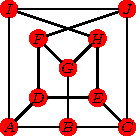
\includegraphics[width=\textwidth, trim={0cm 0cm 0cm 0cm}, clip]{petersen.pdf}
\caption{}
\end{subfigure}\hspace{20pt}
\begin{subfigure}[b]{0.6\textwidth}
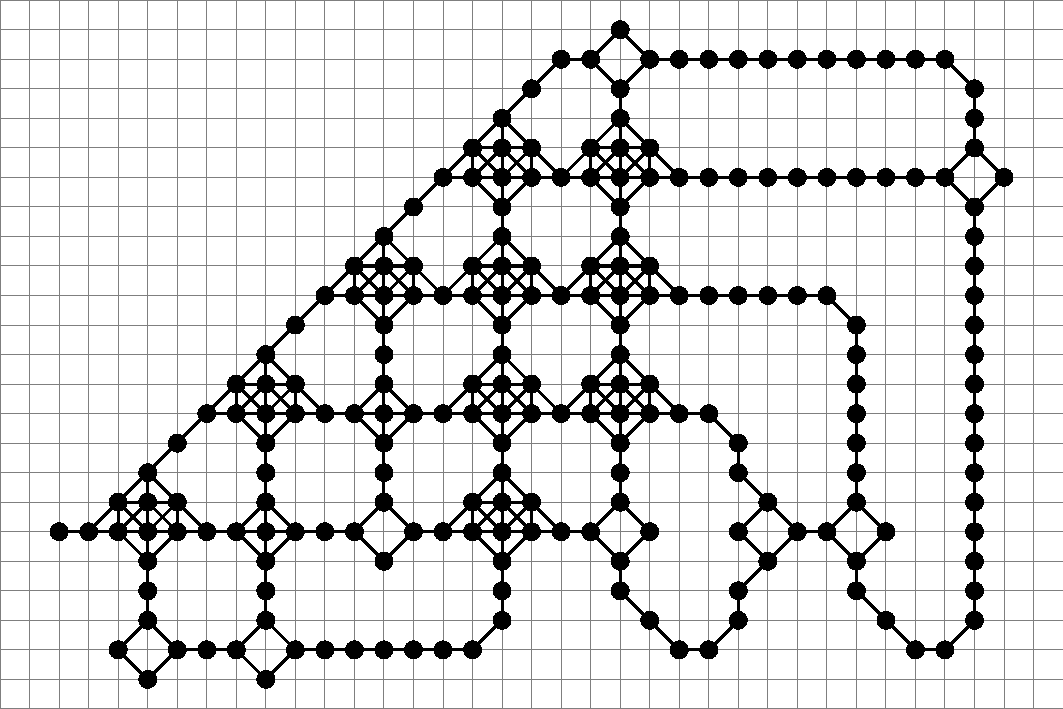
\includegraphics[width=\textwidth, trim={0cm 0cm 0cm 0cm}, clip]{petersen_mapped.pdf}
\caption{}
\end{subfigure}
\caption{(a) The Petersen graph and (b) its diagonal coupled unit disk grid graph embedding.}\label{fig:petersen}
\end{figure}

We also show the proposed mapping scheme is optimal if there is no sub-exponential algorithms for finding the MIS of a general graph, which is, to our knowledge, not found yet.
This work is under the patent now, but the theory part as well as an open source software will be released soon.

\subsection{Future Work}
DUGGs have many nice properties, like the absence overlap gap property in a random instance, the treewidth that scales square root of the size, and can be constant approximated in polynomial time unlike the a general MIS problem.
We also have preliminary simulated annealing result that indicates an average DUGG can be solved in polynomial time, which is too good to be true.
One possible explanation is the mapped graph lives in the hardest corner of the whole set of DUGGs.
I want to study and understand DUGGs more to explain these observations seemingly inconsistent with our previous understanding.
I also want to study the quantum dynamics of the mapped graph under annealing and deepen the understanding of the performance of quantum annealing on this maybe hardest portion of DUGGs.

\section{Summary}
To summarize, the this point in my career, my primary interests are computational hard problems and near term quantum algorithms.
In the future, I want to understand the nature of computational hardness more from the aspects of quantum thermal dynamics and integrability of a quantum system.
Except these research interests, I want to devote half of my time to the help build up the open source scientific software ecosystem.
I believe programming can be used to formalize some part of human knowledge; open source software developing is an integrable, and collaborative way for human to build up the tree of knowledge.
%If there is only one thing I can do in my life, I wish I can grow this tree a bit; given the fact that we are living in a world that open source software developers are never fairly paid, I desperately need a faculty position {\DejaSans ☺}. %, for example, Julia is the best candidate at the moment.
\bibliographystyle{plain}
\bibliography{refs}
\end{document}
